\documentclass[11pt,letterpaper]{article}

\usepackage[margin=1in]{geometry}
\usepackage[T1]{fontenc}
\usepackage{lmodern}
\usepackage{parskip}
\usepackage{microtype}
\usepackage{graphicx}
\usepackage{booktabs}
\usepackage{hyperref}

\setlength{\parindent}{0pt}
\setlength{\parskip}{0.65em}
\pagenumbering{gobble}
\linespread{1.1}

\begin{document}

\begin{center}
{\Large\textbf{Policy Memo}}\\[0.4em]
{\large\textbf{Why Monetary Expansion Is Failing in China --- and What Policymakers Can Do}}\\[0.3em]
{\normalsize Dong Liu \hspace{2em} May 2025}
\end{center}

\noindent\rule{\textwidth}{0.4pt}

\textbf{Executive Summary}

Since 2020, China has experienced weak inflation and episodes of deflation despite rapid expansion of the money supply. This memo argues that the core problem is not insufficient liquidity, but a structural rise in money demand driven by precautionary motives. Heightened uncertainty, weak income expectations, stress in the real estate sector, and erosion of institutional confidence have led households to hold money as a store of safety rather than spend it. As a result, monetary expansion has been absorbed rather than circulated, weakening the link between money growth and prices.

\textbf{Policy implication}: Further monetary easing alone has limited effect in reviving demand. Effective policy must reduce households' incentive to self-insure by restoring confidence and shifting toward direct, household-centered interventions.

\noindent\rule{\textwidth}{0.4pt}

\textbf{The Policy Problem}

China's post-pandemic economy exhibits a clear monetary paradox. Despite rapid growth in the money supply, prices have remained broadly stagnant. Average CPI inflation fell from 2.18 percent in 2016--2020 to 0.77 percent in 2021--2025, with inflation frequently near zero or negative in recent years. At the producer level, deflation has been even more severe: as of May 2025, the Producer Price Index had recorded 32 consecutive months of year-on-year declines, amounting to nearly three years of persistent factory-gate deflation.

\begin{figure}[h]
\centering
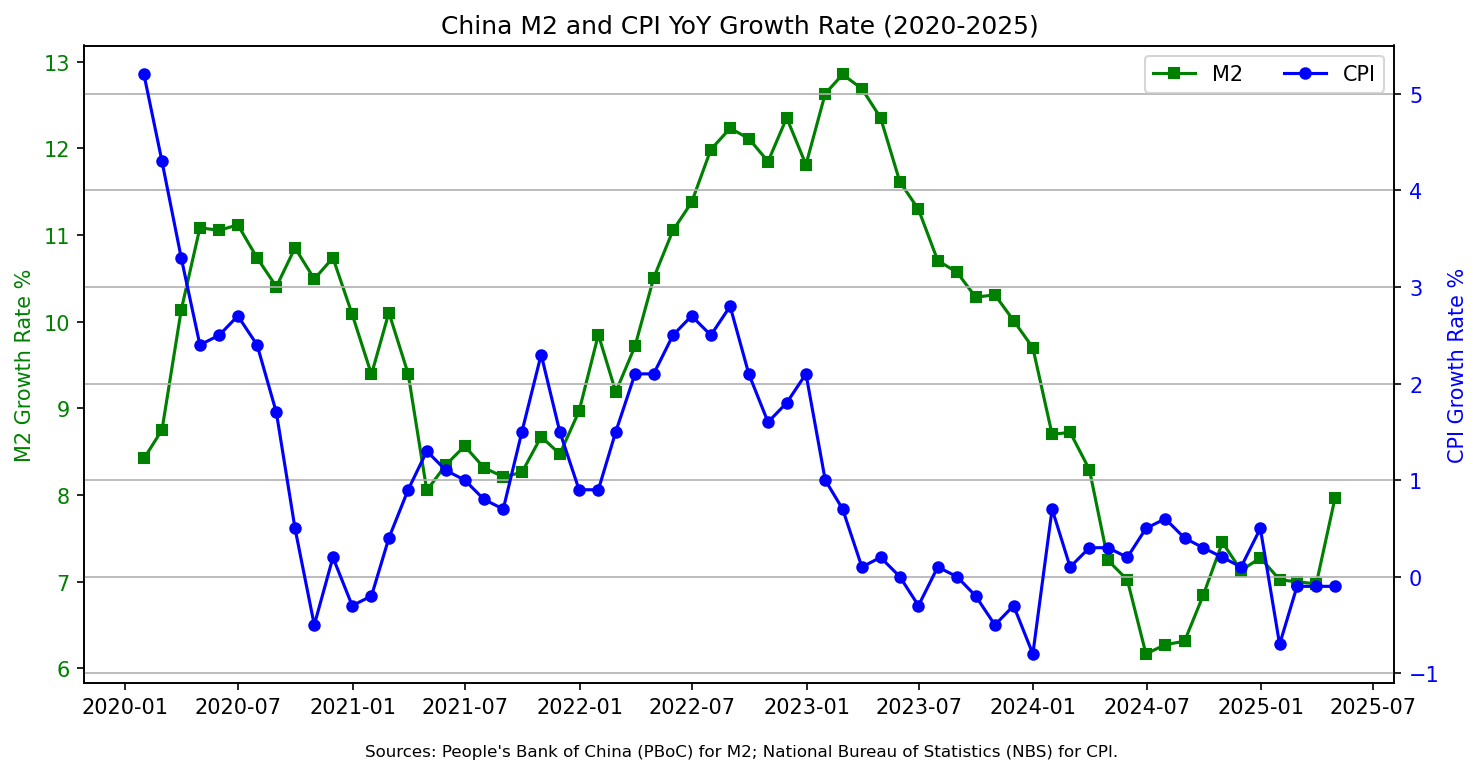
\includegraphics[width=0.92\textwidth]{figure1_m2_cpi.png}
\caption*{\textit{Figure 1: From early 2020 to April 2025, China's broad money supply (M2) rose by over 50\%, while CPI remained subdued and slipped into deflation by mid-2023.}}
\end{figure}

On the surface, monetary expansion appears to be failing to reach the real economy. Liquidity is abundant, yet households and firms have not meaningfully increased borrowing or spending. Policymakers often describe this outcome as a failure of credit transmission. While this characterization captures the immediate symptom, it does not explain why economic agents are choosing to absorb liquidity rather than deploy it through consumption or investment.

\noindent\rule{\textwidth}{0.4pt}

\textbf{Why Credit Transmission Is Failing}

\textit{Precautionary motives dominate household behavior.}

Household behavior has shifted decisively toward liquidity. After 2021, loan growth slowed markedly as households pulled back from borrowing and risk-taking, signaling a move away from consumption and investment toward precautionary saving. This reflects heightened uncertainty rather than constraints on credit supply.

\textit{The real estate shock has weakened wealth and expectations.}

Since 2021, falling home prices, mortgage boycotts, and project delays have undermined confidence in housing as both a store of value and a source of returns. As housing lost its anchoring role in household portfolios, savings increasingly flowed into cash and deposits, raising money demand. Historically, real estate had been the central pillar of household wealth accumulation and investment returns in China.

\textit{Income expectations remain weak amid labor market stress.}

Post-pandemic growth volatility and persistent labor market weakness have weighed heavily on expectations. Youth unemployment peaked above 21 percent in 2023 and remains elevated at 16--18 percent in 2024--2025. These conditions reinforce pessimism about future income and strengthen incentives to self-insure through saving.

\textit{Erosion of institutional confidence has reinforced liquidity preference.}

Prolonged lockdowns during the pandemic, abrupt regulatory changes, and uncertainty around property rights and employment stability have weakened confidence in institutional reliability. As a result, liquidity is held not only for financial reasons, but also as psychological and systemic insurance. In this environment, uncertainty about policy stability has increased the perceived value of holding money, helping explain why precautionary behavior remains elevated despite abundant liquidity.

\noindent\rule{\textwidth}{0.4pt}

\textbf{Why Monetary Expansion Alone Is Insufficient}

Traditional monetary policy assumes that increased liquidity reduces money demand and stimulates spending. When precautionary motives dominate, this mechanism fails. Additional liquidity is absorbed into balance sheets rather than converted into consumption or investment. As a result, further monetary expansion is likely to have limited effect on spending or inflation.

\noindent\rule{\textwidth}{0.4pt}

\textbf{Policy Recommendations}

\textit{Shift from monetary expansion to direct household support.}
Policies should directly reduce households' need to self-insure through targeted fiscal transfers, time-limited consumption incentives, and expanded household-level subsidies.

\textit{Strengthen the social safety net.}
Enhancing unemployment insurance, health coverage, and pension security would reduce precautionary saving and restore the transactional role of money.

\textit{Restore confidence in the housing market.}
Housing completion guarantees and balance-sheet support should prioritize households rather than intermediaries. Credible protection of homeowners' wealth is essential to reversing liquidity hoarding.

\textit{Improve policy credibility and predictability.}
Clear communication, regulatory stability, and fewer abrupt policy reversals are critical to rebuilding institutional trust and anchoring expectations.

\noindent\rule{\textwidth}{0.4pt}

\textbf{Conclusion}

China's deflationary pressures are not primarily the result of insufficient liquidity, but of excess demand for liquidity. Insufficient credit transmission explains the immediate symptoms, but the deeper cause lies in precautionary behavior driven by uncertainty and weakened confidence. Without policies that directly address these structural forces, further monetary expansion alone is unlikely to revive spending or inflation.

\end{document}
